\documentclass{article} 

\usepackage[brazil]{babel}
\usepackage{enumitem}
\usepackage{amsmath}
\usepackage{booktabs}
\usepackage{bm}
\usepackage{float}
\usepackage[margin=2cm]{geometry}
\usepackage{circuitikz}
\usepackage{siunitx}
\usepackage{steinmetz}
\usepackage{amssymb}

\newcommand{\phasor}[2]{%
  #1 \, \phase{\, #2^\circ} \,
}

\newcommand{\ds}{\displaystyle}

% \newcommand{\phasor}[2]{%
%   #1 \, \text{\phase{\, \ang{#2}}} \,
% }

\newcommand{\nle}{%
  \notag \\[8pt]
}

\setlength{\parindent}{0pt}

\title{Modelagem Matemática da Microrrede CC} 
\author{} 
% \date{\today}
\date{}

\begin{document}

\maketitle

\section*{Esquemático da Microrrede}

\begin{figure}[h]
  \centering
  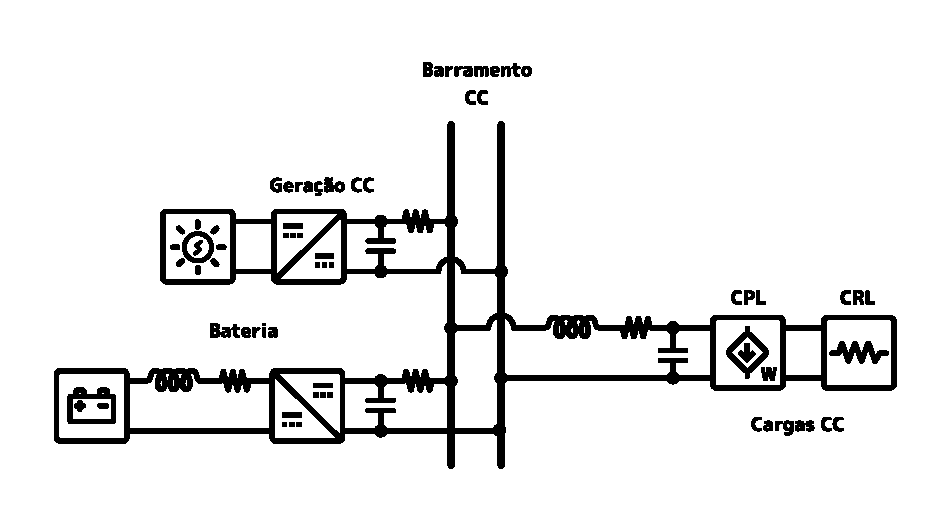
\includegraphics[scale=0.87]{assets/dc_microgrid.eps}
  \caption{Esquemático da Microrrede CC}
  \label{fig:exemplo}
\end{figure}

\subsection*{Modelagem do Subsistema: Geração CC}

O circuito da geração CC está representado abaixo:

\begin{figure}[H]
  \centering
  \begin{circuitikz}[american, scale=0.5, font=\footnotesize]
    \ctikzset{bipoles/length=1cm}
    \draw
    (0,4) to[vsource, v_=$v_G(t)$] (0,0)
    (0,4) to[normal open switch, l=$S_G$] (4,4)
    (4,0) to[diode, l=$D_G$] (4,4)
    (4,4) to[L, l=$L_G$, i_=$i_{L_G}(t)$] (8,4)
    (7,4) to[R, l=$R_{G_1}$] (11,4)
    (11,4) to[C, l=$C_G$, v=$v_{C_G}(t)$] (11,0)
    (11,4) to[R, l=$R_{G_2}$, i_=$i_{G}(t)$] (15,4)

    (15,4) to[short, -o] (16,4)
    (0,0) to[short, -o] (16,0)

    (16,4) to[open, v=$v_E(t)$] (16,0)
    ;
  \end{circuitikz}
\end{figure}

Aplicando a LKT na segunda malha a partir da esquerda, obtemos:
\begin{gather}
  d_G(t) v_G(t) - L_G \dot{i}_{L_G} - R_{G_1} i_{L_G}(t) - v_{C_G}(t) = 0 \nle
  \dot{i}_{L_G} = - \frac{R_{G_1}}{L_G} i_{L_G}(t) - \frac{1}{L_G} v_{C_G}(t) + \frac{v_G(t)}{L_G} d_G(t)
\end{gather}

Aplicando a LKC, obtemos:
\begin{gather}
  i_{L_G}(t) = C_G \dot{v}_{C_G} + i_G(t)
\end{gather}

Têm-se que, $i_G(t) = \frac{v_{C_G}(t) - v_E(t)}{R_{G_2}}$. Logo,
\begin{gather}
  i_{L_G}(t) = C_G \dot{v}_{C_G} + \frac{1}{R_{G_2}}v_{C_G}(t) - \frac{1}{R_{G_2}} v_E(t) \nle
  i_{L_G}(t) = C_G \dot{v}_{C_G} + \frac{1}{R_{G_2}}v_{C_G}(t) - \frac{1}{R_{G_2}} v_E(t) \nle
  \dot{v}_{C_G} = \frac{1}{C_G} i_{L_G}(t) - \frac{1}{R_{G_2}C_G }v_{C_G}(t) + \frac{1}{R_{G_2} C_G} v_E(t)
\end{gather}

Portanto, o modelo do subsistema da geração é:
\begin{gather}
  \begin{cases}
    \dot{i}_{L_G} = \displaystyle - \frac{R_{G_1}}{L_G} i_{L_G}(t) - \frac{1}{L_G} v_{C_G}(t) + \frac{v_G(t)}{L_G} d_G(t) \\[8pt]
    \dot{v}_{C_G} = \displaystyle \frac{1}{C_G} i_{L_G}(t) - \frac{1}{R_{G_2}C_G }v_{C_G}(t) + \frac{1}{R_{G_2} C_G} v_E(t)
  \end{cases}
\end{gather}

\vspace*{8pt}
\subsection*{Modelagem do Subsistema: Bateria}

O circuito que representa o subsistema da bateria está apresentado abaixo:

\begin{figure}[H]
  \centering
  \begin{circuitikz}[american, scale=0.5, font=\footnotesize]
    \ctikzset{bipoles/length=1cm}
    \draw
    (0,4) to[battery, v_=$v_B(t)$] (0,0)
    (0,4) to[L,l=$L_{B}$, i_=$i_{L_B}(t)$] (4,4)
    (3,4) to[R,l=$R_{B_1}$] (7,4)
    (7,0) to[normal closed switch, l=$S_{B_1}$] (7,4)
    (7,4) to[normal open switch, l=$S_{B_2}$] (11,4)
    (11,4) to[C, l=$C_{B}$, v=$v_{C_B}(t)$] (11,0)
    (11,4) to[R,l=$R_{B_2}$, i=$i_B(t)$, -o] (15,4)
    (0,0) to[short, -o] (15,0)
    (15,4) to[open, v=$v_E(t)$] (15,0)
    ;
  \end{circuitikz}
\end{figure}

\subsubsection*{Para $S_{B_1}$ fechada e $S_{B_2}$ aberta: $d_B(t) \cdot T_se$}

Aplicando a LKT na malha mais a esquerda, obtemos:
\begin{gather}
  v_B(t) - L_B \dot{i}_{L_B} - R_{B_1} i_{L_B} (t) = 0 \nle
  \dot{i}_{L_B} = - \frac{R_{B_1}}{L_B} i_{L_B}(t) + \frac{1}{L_B} v_B(t)
\end{gather}

Aplicando a LKC na malha mais a direita, tém-se:
\begin{gather}
  i_B(t) + C_B \dot{v}_{C_B}(t) = 0
\end{gather}

Como $i_B(t) = \frac{v_{C_B}(t) - v_E(t)}{R_{B_2}}$, têm-se:
\begin{gather}
  \frac{v_{C_B}(t)}{R_{B_2}} - \frac{v_E(t)}{R_{B_2}} + C_B \dot{v}_{C_B}(t) = 0 \nle
  \dot{v}_{C_B}(t) = - \frac{1}{R_{B_2} C_B} v_{C_B}(t) + \frac{1}{R_{B_2} C_B} v_{E}(t)
\end{gather}

Assim, neste modo, têm-se:
\begin{gather}
  \begin{cases}
    \dot{i}_{L_B} = \displaystyle - \frac{R_{B_1}}{L_B} i_{L_B}(t) + \frac{1}{L_B} v_B(t) \\[8pt]
    \dot{v}_{C_B}(t) = \displaystyle - \frac{1}{R_{B_2} C_B} v_{C_B}(t) + \frac{1}{R_{B_2} C_B} v_{E}(t)
  \end{cases}
\end{gather}

\vspace*{8pt}
\subsubsection*{Para $S_{B_1}$ aberta e $S_{B_2}$ fechada: $\left[1 - d_B(t)\right] \cdot T_s$}

Aplicando a LKT, obtemos:
\begin{gather}
  v_B(t) - L_B \dot{i}_{L_B} - R_{B_1} i_{L_B} (t) - v_{C_B} (t)= 0 \nle
  \dot{i}_{L_B} = - \frac{R_{B_1}}{L_B} i_{L_B}(t) - \frac{1}{L_B} v_{C_B} (t) + \frac{1}{L_B} v_B(t)
\end{gather}

Aplicando a LKC, obtemos:
\begin{gather}
  i_{L_B}(t) = C_B v_{C_B}(t) + i_B(t) \nle
  i_{L_B}(t) = C_B \dot{v}_{C_B}(t) +  \frac{v_{C_B}(t)}{R_{B_2}} - \frac{v_E(t)}{R_{B_2}} \nle
  \dot{v}_{C_B}(t) =  \frac{1}{C_B} i_{L_B}(t) - \frac{1}{R_{B_2}C_B} v_{C_B}(t) + \frac{1}{R_{B_2} C_B} v_E(t)
\end{gather}

Assim, neste modo, têm-se:
\begin{gather}
  \begin{cases}
    \dot{i}_{L_B} = \displaystyle - \frac{R_{B_1}}{L_B} i_{L_B}(t) - \frac{1}{L_B} v_{C_B} (t) + \frac{1}{L_B} v_B(t) \\[8pt]
    \dot{v}_{C_B} = \displaystyle \frac{1}{C_B} i_{L_B}(t) - \frac{1}{R_{B_2}C_B} v_{C_B}(t) + \frac{1}{R_{B_2} C_B} v_E(t)
  \end{cases}
\end{gather}

\vspace*{8pt}
\subsubsection*{Modelo Médio Completo}
A equação completa da dinâmica da corrente ${i}_{L_B}(t)$ é:
\begin{gather}
  \dot{i}_{L_B} = \left[- \frac{R_{B_1}}{L_B} i_{L_B}(t) + \frac{1}{L_B} v_B(t)\right] d_B(t) + \left[- \frac{R_{B_1}}{L_B} i_{L_B}(t) - \frac{1}{L_B} v_{C_B} (t) + \frac{1}{L_B} v_B(t)\right] \left[1 - d_B(t)\right] \nle
  \dot{i}_{L_B} = - \frac{R_{B_1}}{L_B} i_{L_B}(t) - \frac{1}{L_B} v_{C_B} (t) + \frac{1}{L_B} \left[1 - d_B(t)\right] v_B(t)
\end{gather}

E da tensão,
\begin{gather}
  \dot{v}_{C_B}(t) = \left[- \frac{1}{R_{B_2} C_B} v_{C_B}(t) + \frac{1}{R_{B_2} C_B} v_{E}(t)\right] d_B(t) + \left[\frac{1}{C_B} i_{L_B}(t) - \frac{1}{R_{B_2}C_B} v_{C_B}(t) + \frac{1}{R_{B_2} C_B} v_E(t)\right] \left[1 - d_B(t)\right] \nle
  \dot{v}_{C_B} = \frac{1}{C_B} \left[1 - d_B(t)\right] i_{L_B}(t) - \frac{1}{R_{B_2}C_B} v_{C_B}(t) + \frac{1}{R_{B_2} C_B} v_E(t)
\end{gather}

Portanto, o modelo dinâmico do subsistema da bateria é:
\begin{gather}
  \begin{cases}
    \dot{i}_{L_B} = \displaystyle - \frac{R_{B_1}}{L_B} i_{L_B}(t) - \frac{1}{L_B} v_{C_B} (t) + \frac{1}{L_B} \left[1 - d_B(t)\right] v_B(t) \\[8pt]
    \dot{v}_{C_B} = \displaystyle \frac{1}{C_B} \left[1 - d_B(t)\right] i_{L_B}(t) - \frac{1}{R_{B_2}C_B} v_{C_B}(t) + \frac{1}{R_{B_2} C_B} v_E(t)
  \end{cases}
\end{gather}

\vspace*{8pt}
\subsection*{Modelagem do Subsistema: Cargas}

O circuito que representa as duas cargas conectadas a redes, a CPL e a CRL, é:

\begin{figure}[H]
  \centering
  \begin{circuitikz}[american, scale=0.5, font=\footnotesize]
    \ctikzset{bipoles/length=1cm}
    \draw
    (0,4) to[open, v_=$v_E(t)$, o-o] (0,0)
    (0,4) to[L,l=$L_{K}$, i_=$i_{L_K}(t)$] (4,4)
    (3,4) to[R,l=$R_{K}$] (7,4)
    (7,4) to[C, l=$C_{K}$, v=$v_{C_K}(t)$] (7,0)
    (11,4) to[controlled current source, l={$i(t) = \frac{P_{cpl}(t)}{v_{C_K}(t)}$}] (11,0)
    (0,0) to[short] (16,0)
    (7,4) to[short] (16,4)
    (16,4) to[R, l=$R_{rcl}$] (16,0)
    ;
  \end{circuitikz}
\end{figure}

Aplicando a LKT na malha mais a esquerda, têm-se:
\begin{gather}
  v_E(t) - L_K \dot{i}_{L_K} - R_K i_{L_K}(t) - v_{C_K}(t) = 0 \nle
  \dot{i}_{L_K} = - \frac{R_K}{L_K} i_{L_K}(t) - \frac{1}{L_K} v_{C_K}(t) + \frac{1}{L_K} v_E(t)
\end{gather}

Aplicando a LKC, obtemos:
\begin{gather}
  i_{L_K} = C_K \dot{v}_{C_K} + \frac{P_{cpl}(t)}{v_{C_K}(t)} + \frac{v_{C_K}(t)}{R_{crl}} \nle
  \dot{v}_{C_K} = \frac{1}{C_K} i_{L_K} - \frac{1}{R_{crl} C_K} v_{C_K}(t) - \frac{1}{C_K} \frac{P_{cpl}(t)}{v_{C_K}(t)}
\end{gather}

Portanto, o modelo dinâmico do subsistema das cargas é:
\begin{gather}
  \begin{cases}
    \dot{i}_{L_K} = \displaystyle - \frac{R_K}{L_K} i_{L_K}(t) - \frac{1}{L_K} v_{C_K}(t) + \frac{1}{L_K} v_E(t) \\[8pt]
    \dot{v}_{C_K} = \displaystyle \frac{1}{C_K} i_{L_K} - \frac{1}{R_{crl} C_K} v_{C_K}(t) - \frac{1}{C_K} \frac{P_{cpl}(t)}{v_{C_K}(t)}
  \end{cases}
\end{gather}

\subsection*{Centralização dos Modelos}

Do esquemático, têm-se que:
\begin{gather}
  i_G(t) + i_B(t) = i_{L_K}(t) \nle
  \frac{1}{R_{G_2}} v_{C_G}(t) - \frac{1}{R_{G_2}} v_E(t) +
  \frac{1}{R_{B_2}} v_{C_B}(t) - \frac{1}{R_{B_2}} v_E(t) =  i_{L_K}(t) \nle
  i_G(t) + i_B(t) = i_{L_K}(t) \nle
  \frac{1}{R_{G_2}} v_{C_G}(t) + \frac{1}{R_{B_2}} v_{C_B}(t)
  - \left[\frac{1}{R_{G_2}} + \frac{1}{R_{B_2}}\right] v_E(t) =  i_{L_K}(t) \nle
  v_E(t) = - \frac{1}{\displaystyle \frac{1}{R_{G_2}} + \frac{1}{R_{B_2}}} i_{L_K}(t) + \frac{1}{R_{G_2} \left[\frac{1}{R_{G_2}} + \frac{1}{R_{B_2}}\right]} v_{C_G}(t) + \frac{1}{R_{B_2} \left[\frac{1}{R_{G_2}} + \frac{1}{R_{B_2}}\right]} v_{C_B}(t) \nle
  v_E(t) = - \frac{R_{G_2}R_{B_2}}{R_{G_2} + R_{B_2}} i_{L_K}(t) + \frac{R_{G_2}R_{B_2}}{R_{G_2} \left(R_{G_2} + R_{B_2}\right)} v_{C_G}(t) + \frac{R_{G_2}R_{B_2}}{R_{B_2} \left(R_{G_2} + R_{B_2}\right)}  v_{C_B}(t) \nle
  v_E(t) = - \frac{R_{G_2}R_{B_2}}{R_{G_2} + R_{B_2}} i_{L_K}(t) + \frac{R_{B_2}}{R_{G_2} + R_{B_2}} v_{C_G}(t) + \frac{R_{G_2}}{R_{G_2} + R_{B_2}}  v_{C_B}(t) \nle
  v_E(t) = - R_{G_2} R_{E_1} i_{L_K}(t) + R_{E_1} v_{C_G}(t) + R_{E_2} v_{C_B}(t)
\end{gather}

onde, $R_{E_1} = \displaystyle \frac{R_{B_2}}{R_{G_2} + R_{B_2}}$ e $R_{E_2} = \displaystyle \frac{R_{G_2}}{R_{G_2} + R_{B_2}}.$
\vspace*{2pt}
Assim, o modelo centralizado é:

\begin{gather}
  \begin{cases}
    \dot{i}_{L_G} = \ds - \frac{R_{G_1}}{L_G} i_{L_G}(t) - \frac{1}{L_G} v_{C_G}(t) + \frac{v_G(t)}{L_G} d_G(t)                                                                                                \\[12pt]
    \dot{i}_{L_B} = \ds - \frac{R_{B_1}}{L_B} i_{L_B}(t) - \frac{1}{L_B} v_{C_B} (t) + \frac{1}{L_B} \left[1 - d_B(t)\right] v_B(t)                                                                            \\[12pt]
    \dot{i}_{L_K} = \ds - \frac{R_K + R_{G_2} R_{E_1}}{L_K} i_{L_K}(t) - \frac{1}{L_K} v_{C_K}(t)  + \frac{R_{E_1}}{L_K} v_{C_G}(t) + \frac{R_{E_2}}{L_K} v_{C_B}(t)                                           \\[12pt]
    \dot{v}_{C_G} = \ds \frac{1}{C_G} i_{L_G}(t) - \frac{1 - R_{E_1}}{C_G R_{G_2}} v_{C_G}(t) - \frac{R_{E_1}}{C_G} i_{L_K}(t) + \frac{R_{E_2}}{R_{G_2} C_G} v_{C_B}(t)                                        \\[12pt]
    \dot{v}_{C_B} = \ds \frac{1}{C_B} \left[1 - d_B(t)\right] i_{L_B}(t) - \frac{1 - R_{E_2}}{R_{B_2}C_B} v_{C_B}(t) - \frac{R_{G_2} R_{E_1}}{R_{B_2} C_B} i_{L_K}(t) + \frac{R_{E_1}}{R_{B_2} C_B} v_{C_G}(t) \\[12pt]
    \dot{v}_{C_K} = \ds \frac{1}{C_K} i_{L_K} - \frac{1}{R_{crl} C_K} v_{C_K}(t) - \frac{1}{C_K} \frac{P_{cpl}(t)}{v_{C_K}(t)}
  \end{cases}
\end{gather}

No espaço de estados, temos:
\begin{gather}
  \begin{bmatrix}
    \dot{i}_{L_G} \\[12pt] \dot{i}_{L_B} \\[12pt] \dot{i}_{L_K} \\[12pt]
    \dot{v}_{C_G} \\[12pt] \dot{v}_{C_B} \\[12pt] \dot{v}_{C_K}
  \end{bmatrix} =
  \begin{bmatrix}
    \ds - \frac{R_{G_1}}{L_G} & 0                         & 0                                         & \ds - \frac{1}{L_G}                  & 0                                    & 0                           \\[12pt]
    0                         & \ds - \frac{R_{B_1}}{L_B} & 0                                         & 0                                    & \ds - \frac{1}{L_B}                  & 0                           \\[12pt]
    0                         & 0                         & - \ds \frac{R_K + R_{G_2} R_{E_1}}{L_K}   & \ds \frac{R_{E_1}}{L_K}              & \ds \frac{R_{E_2}}{L_K}              & - \ds \frac{1}{L_K}         \\[12pt]
    \ds \frac{1}{C_G}         & 0                         & \ds - \frac{R_{E_1}}{C_G}                 & \ds - \frac{1 - R_{E_1}}{R_{G_2}C_G} & \ds \frac{R_{E_2}}{R_{G_2}C_G}       & 0                           \\[12pt]
    0                         & \ds \frac{1}{C_B}         & \ds - \frac{R_{G_2} R_{E_1}}{R_{B_2} C_B} & \ds \frac{R_{E_1}}{R_{B_2} C_B}      & \ds - \frac{1 - R_{E_2}}{R_{B_2}C_B} & 0                           \\[12pt]
    0                         & 0                         & \ds \frac{1}{C_K}                         & 0                                    & 0                                    & \ds - \frac{1}{R_{crl} C_K}
  \end{bmatrix}
  \begin{bmatrix}
    i_{L_G}(t) \\[12pt] i_{L_B}(t) \\[12pt] i_{L_K}(t) \\[12pt]
    v_{C_G}(t) \\[12pt] v_{C_B}(t) \\[12pt] v_{C_K}(t)
  \end{bmatrix} \notag \\[12pt] +
  \begin{bmatrix}
    \ds \frac{v_G(t)}{L_G} & 0                 & 0                            & 0                              \\[12pt]
    0                      & \ds \frac{1}{L_B} & \ds - \frac{v_B(t)}{L_B}     & 0                              \\[12pt]
    0                      & 0                 & 0                            & 0                              \\[12pt]
    0                      & 0                 & 0                            & 0                              \\[12pt]
    0                      & 0                 & - \ds \frac{i_{L_B}(t)}{C_B} & 0                              \\[12pt]
    0                      & 0                 & 0                            & - \ds \frac{1}{C_K v_{C_K}(t)} \\[12pt]
  \end{bmatrix}
  \begin{bmatrix}
    d_G(t) \\ v_B(t) \\ d_B(t) \\ P_{cpl}(t)
  \end{bmatrix}
\end{gather}

\begin{equation}
  v_E(t) =
  \begin{bmatrix}
    0 & 0 & 0                 & 0       & 0       & 0 \\[12pt]
    0 & 0 & 0                 & 0       & 0       & 0 \\[12pt]
    0 & 0 & - R_{G_2} R_{E_1} & 0       & 0       & 0 \\[12pt]
    0 & 0 & 0                 & R_{E_1} & 0       & 0 \\[12pt]
    0 & 0 & 0                 & 0       & R_{E_2} & 0 \\[12pt]
    0 & 0 & 0                 & 0       & 0       & 0 \\[12pt]
  \end{bmatrix}
  \begin{bmatrix}
    i_{L_G}(t) \\[12pt] i_{L_B}(t) \\[12pt] i_{L_K}(t) \\[12pt]
    v_{C_G}(t) \\[12pt] v_{C_B}(t) \\[12pt] v_{C_K}(t)
  \end{bmatrix}
\end{equation}

\subsection*{Translação}

Parcelando os estados e as entradas do sistema em termos fixos e em termos variantes no tempo, obtemos:

\begin{gather}
  i_{L_G}(t) = i_{L_G}^o + \delta i_{L_G}(t) \nle
  i_{L_B}(t) = i_{L_B}^o + \delta i_{L_B}(t) \nle
  i_{L_K}(t) = i_{L_K}^o + \delta i_{L_K}(t) \nle
  v_{C_G}(t) = v_{C_G}^o + \delta v_{C_G}(t) \nle
  v_{C_B}(t) = v_{C_B}^o + \delta v_{C_B}(t) \nle
  v_{C_K}(t) = v_{C_K}^o + \delta v_{C_K}(t) \nle
  d_G(t) = d_G^o + \delta d_G(t) \nle
  d_B(t) = d_B^o + \delta d_B(t) \nle
  v_B(t) = v_B^o + \delta v_B(t) \nle
  P_{cpl}(t) = P_{cpl}^o + \delta P_{cpl}(t)
\end{gather}

\textbf{\textit{Corrente $i_{L_G}$ transladada}} \vspace*{12pt}

Para $\dot{i}_{L_G}$, têm-se:
\begin{gather}
  - \frac{R_{G_1}}{L_G} i_{L_G}^o - \frac{1}{L_G} v_{C_G}^o + \frac{v_G(t)}{L_G} d_G^o = 0 \nle
  - R_{G_1} i_{L_G}^o - v_{C_G}^o + v_G(t) d_G^o = 0 \nle
  d_G^o = \frac{R_{G_1}}{v_G(t)} i_{L_G}^o + \frac{1}{v_G(t)} v_{C_G}^o
\end{gather}

Substituindo, obtemos:
\begin{gather}
  \dot{i}_{L_G} = - \frac{R_{G_1}}{L_G} i_{L_G}(t) - \frac{1}{L_G} v_{C_G}(t) + \frac{v_G(t)}{L_G} d_G(t) \nle
  \delta \dot{i}_{L_G} = - \frac{R_{G_1}}{L_G} \left[i_{L_G}^o + \delta i_{L_G}(t)\right]
  - \frac{1}{L_G} \left[v_{C_G}^o + \delta v_{C_G}(t)\right]
  + \frac{v_G(t)}{L_G} \left[\frac{R_{G_1}}{v_G(t)} i_{L_G}^o + \frac{1}{v_G(t)} v_{C_G}^o + \delta d_G(t)\right] \nle
  \delta \dot{i}_{L_G} = - \frac{R_{G_1}}{L_G} \delta i_{L_G}(t) - \frac{1}{L_G} \delta v_{C_G}(t) + \frac{v_B(t)}{L} \delta d_G(t)
\end{gather}

\textbf{\textit{Corrente $i_{L_B}$ transladada}} \vspace*{12pt}

Para $\dot{i}_{L_B}$, têm-se:
\begin{gather}
  - \frac{R_{B_1}}{L_B} i_{L_B}^o - \frac{1}{L_B} v_{C_B} ^o + \frac{1}{L_B} \left[1 - d_B^o\right] v_B^o = 0 \nle
  d_B^o = -\frac{R_{B_1}}{v_B^o} i_{L_B}^o - \frac{1}{v_B^o} v_{C_B}^o + 1
\end{gather}

Substituindo, obtemos:
\begin{gather}
  \delta \dot{i}_{L_B} = - \frac{R_{B_1}}{L_B} i_{L_B}(t) - \frac{1}{L_B} v_{C_B} (t) + \frac{1}{L_B} \left[1 - d_B(t)\right] v_B(t) \nle
  \delta \dot{i}_{L_B} = - \frac{R_{B_1}}{L_B} \left[i_{L_B}^o + \delta i_{L_B}(t)\right]
  - \frac{1}{L_B} \left[v_{C_B}^o + \delta v_{C_B} (t)\right]
  + \frac{1}{L_B} \left[\frac{R_{B_1}}{v_B^o} i_{L_B}^o + \frac{1}{v_B^o} v_{C_B}^o - \delta d_B(t)\right]
  \left[v_B^o + \delta v_B(t)\right] \nle
  \delta \dot{i}_{L_B} = - \frac{v_B^o}{L_B} \delta d_B(t) - \frac{R_{B_1}}{L_B} \delta i_{L_B}(t)
  - \frac{1}{L_B} \delta v_{C_B}(t) - \frac{1}{L_B} \delta d_B(t) \delta v_B(t)
  + \frac{R_{B_1} i_{L_B}^o + v_{C_B}^o}{L_B v_B^o} \delta v_B(t)
\end{gather}

\textbf{\textit{Corrente $i_{L_K}$ transladada}} \vspace*{12pt}

Para $\dot{i}_{L_K}$, têm-se:
\begin{gather}
  - \frac{R_K + R_{G_2} R_{E_1}}{L_K} i_{L_K}^o - \frac{1}{L_K} v_{C_K}^o  + \frac{R_{E_1}}{L_K} v_{C_G}^o + \frac{R_{E_2}}{L_K} v_{C_B}^o = 0 \nle
  i_{L_K}^o = - \frac{1}{R_K + R_{G_2} R_{E_1}} v_{C_K}^o  + \frac{R_{E_1}}{R_K + R_{G_2} R_{E_1}} v_{C_G}^o + \frac{R_{E_2}}{R_K + R_{G_2} R_{E_1}} v_{C_B}^o
\end{gather}

Substituindo, obtemos:
\begin{gather}
  \dot{i}_{L_K} = - \frac{R_K + R_{G_2} R_{E_1}}{L_K} i_{L_K}(t) - \frac{1}{L_K} v_{C_K}(t)  + \frac{R_{E_1}}{L_K} v_{C_G}(t) + \frac{R_{E_2}}{L_K} v_{C_B}(t) \nle
  \delta \dot{i}_{L_K} = - \frac{R_K + R_{G_2} R_{E_1}}{L_K} \left[i_{L_K}^o + \delta i_{L_K}(t) \right] - \frac{1}{L_K} \left[v_{C_K}^o + \delta v_{C_K}(t)\right]  + \frac{R_{E_1}}{L_K} \left[v_{C_G}^o + \delta v_{C_G}(t)\right] + \frac{R_{E_2}}{L_K} \left[v_{C_B}^o + \delta v_{C_B}(t)\right] \nle
  \delta \dot{i}_{L_K} = \frac{R_{E_1}}{L_K} \delta v_{C_G}(t) - \frac{R_K+R_{G_2}R_{E_1}}{L_K} \delta i_{L_K}(t)
  - \frac{1}{L_K} \delta v_{C_K}(t) + \frac{R_{E_2}}{L_K} \delta v_{C_B}(t)
\end{gather}

\textbf{\textit{Tensão $v_{C_G}$ transladada}} \vspace*{12pt}

Para $\dot{v}_{C_G}$, têm-se:
\begin{gather}
  \frac{1}{C_G} i_{L_G}^o - \frac{1 - R_{E_1}}{C_G R_{G_2}} v_{C_G}^o - \frac{R_{E_1}}{C_G} i_{L_K}^o + \frac{R_{E_2}}{R_{G_2} C_G} v_{C_B}^o = 0 \nle
  i_{L_G}^o = \frac{1 - R_{E_1}}{R_{G_2}} v_{C_G}^o + R_{E_1} i_{L_K}^o - \frac{R_{E_2}}{R_{G_2}} v_{C_B}^o
\end{gather}

Substituindo, obtemos:
\begin{gather}
  \dot{v}_{C_G} = \frac{1}{C_G} i_{L_G}(t) - \frac{1 - R_{E_1}}{C_G R_{G_2}} v_{C_G}(t) - \frac{R_{E_1}}{C_G} i_{L_K}(t) + \frac{R_{E_2}}{R_{G_2} C_G} v_{C_B}(t) \nle
  \delta \dot{v}_{C_G} = \frac{1}{C_G} \left[i_{L_G}^o + \delta i_{L_G}(t)\right]
  - \frac{1 - R_{E_1}}{C_G R_{G_2}} \left[v_{C_G}^o + \delta v_{C_G}(t) \right]
  - \frac{R_{E_1}}{C_G} \left[i_{L_K}^o + \delta i_{L_K}(t)\right]
  + \frac{R_{E_2}}{R_{G_2} C_G} \left[v_{C_B}^o + \delta v_{C_B}(t)\right] \nle
  \delta \dot{v}_{C_G} = \frac{R_{E_1} - 1}{R_{G_2} C_G} \delta v_{C_G}(t)
  - \frac{R_{E_1}}{C_G} \delta i_{L_K}(t)
  + \frac{R_{E_2}}{R_{G_2} C_G} \delta v_{C_B}(t) + \frac{1}{C_G} \delta i_{L_G}(t)
\end{gather}

\textbf{\textit{Tensão $v_{C_B}$ transladada}} \vspace*{12pt}

Para $\dot{v}_{C_B}$, têm-se:
\begin{gather}
  \frac{1}{C_B} \left[1 - d_B^o\right] i_{L_B}^o - \frac{1 - R_{E_2}}{R_{B_2}C_B} v_{C_B}^o - \frac{R_{G_2} R_{E_1}}{R_{B_2} C_B} i_{L_K}^o + \frac{R_{E_1}}{R_{B_2} C_B} v_{C_G}^o = 0 \nle
  i_{L_B}^o = \frac{1 - R_{E_2}}{R_{B_2} \left[1 - d_B^o\right]} v_{C_B}^o + \frac{R_{G_2} R_{E_1}}{R_{B_2} \left[1 - d_B^o\right]} i_{L_K}^o - \frac{R_{E_1}}{R_{B_2} \left[1 - d_B^o\right]} v_{C_G}^o
\end{gather}

Substituindo, obtemos:
\begin{gather*}
  \dot{v}_{C_B} = \frac{1}{C_B} \left[1 - d_B(t)\right] i_{L_B}(t) - \frac{1 - R_{E_2}}{R_{B_2}C_B} v_{C_B}(t) - \frac{R_{G_2} R_{E_1}}{R_{B_2} C_B} i_{L_K}(t) + \frac{R_{E_1}}{R_{B_2} C_B} v_{C_G}(t)
\end{gather*}
\begin{multline*}
  \delta \dot{v}_{C_B} = \frac{1}{C_B} \left[1 - d_B^o - \delta d_B(t)\right] \left[i_{L_B}^o + \delta i_{L_B}(t) \right]
  - \frac{1 - R_{E_2}}{R_{B_2}C_B} \left[v_{C_B}^o + \delta v_{C_B}(t)\right] \\
  - \frac{R_{G_2} R_{E_1}}{R_{B_2} C_B} \left[i_{L_K}^o + \delta i_{L_K}(t)\right]
  + \frac{R_{E_1}}{R_{B_2} C_B} \left[v_{C_G}^o + \delta v_{C_G}(t)\right]
\end{multline*}
\begin{multline*}
  \delta \dot{v}_{C_B} = \frac{1}{C_B} \left[1 - d_B^o\right] \left[i_{L_B}^o + \delta i_{L_B}(t) \right]
  - \delta d_B(t) \left[i_{L_B}^o + \delta i_{L_B}(t) \right]
  - \frac{1 - R_{E_2}}{R_{B_2}C_B} \left[v_{C_B}^o + \delta v_{C_B}(t)\right] \\
  - \frac{R_{G_2} R_{E_1}}{R_{B_2} C_B} \left[i_{L_K}^o + \delta i_{L_K}(t)\right]
  + \frac{R_{E_1}}{R_{B_2} C_B} \left[v_{C_G}^o + \delta v_{C_G}(t)\right]
\end{multline*}
\begin{multline*}
  \delta \dot{v}_{C_B} = \frac{1}{C_B} \left[1 - d_B^o\right] i_{L_B}^o + \frac{1}{C_B} \left[1 - d_B^o\right] \delta i_{L_B}(t)
  - \delta d_B(t) \left[i_{L_B}^o + \delta i_{L_B}(t) \right]
  - \frac{1 - R_{E_2}}{R_{B_2}C_B} \left[v_{C_B}^o + \delta v_{C_B}(t)\right] \\
  - \frac{R_{G_2} R_{E_1}}{R_{B_2} C_B} \left[i_{L_K}^o + \delta i_{L_K}(t)\right]
  + \frac{R_{E_1}}{R_{B_2} C_B} \left[v_{C_G}^o + \delta v_{C_G}(t)\right]
\end{multline*}
\begin{multline*}
  \delta \dot{v}_{C_B} = \frac{1}{C_B} \left[1 - d_B^o\right] \left[\frac{1 - R_{E_2}}{R_{B_2} \left[1 - d_B^o\right]} v_{C_B}^o + \frac{R_{G_2} R_{E_1}}{R_{B_2} \left[1 - d_B^o\right]} i_{L_K}^o - \frac{R_{E_1}}{R_{B_2} \left[1 - d_B^o\right]} v_{C_G}^o\right] \\
  + \frac{1}{C_B} \left[1 - d_B^o\right] \delta i_{L_B}(t)
  - \delta d_B(t) \left[i_{L_B}^o + \delta i_{L_B}(t) \right]
  - \frac{1 - R_{E_2}}{R_{B_2}C_B} \left[v_{C_B}^o + \delta v_{C_B}(t)\right] \\
  - \frac{R_{G_2} R_{E_1}}{R_{B_2} C_B} \left[i_{L_K}^o + \delta i_{L_K}(t)\right]
  + \frac{R_{E_1}}{R_{B_2} C_B} \left[v_{C_G}^o + \delta v_{C_G}(t)\right]
\end{multline*}
\begin{multline*}
  \delta \dot{v}_{C_B} = \frac{1 - R_{E_2}}{R_{B_2}C_B} v_{C_B}^o + \frac{R_{G_2} R_{E_1}}{R_{B_2}C_B} i_{L_K}^o - \frac{R_{E_1}}{R_{B_2}C_B} v_{C_G}^o
  + \frac{1}{C_B} \left[1 - d_B^o\right] \delta i_{L_B}(t)
  - \delta d_B(t) \left[i_{L_B}^o + \delta i_{L_B}(t) \right] \\
  - \frac{1 - R_{E_2}}{R_{B_2}C_B} \left[v_{C_B}^o + \delta v_{C_B}(t)\right]
  - \frac{R_{G_2} R_{E_1}}{R_{B_2} C_B} \left[i_{L_K}^o + \delta i_{L_K}(t)\right]
  + \frac{R_{E_1}}{R_{B_2} C_B} \left[v_{C_G}^o + \delta v_{C_G}(t)\right]
\end{multline*}
\begin{multline}
  \delta \dot{v}_{C_B} = - \frac{1 - R_{E_2}}{R_{B_2}C_B} \delta v_{C_B}(t)
  - \frac{R_{G_2} R_{E_1}}{R_{B_2}C_B} \delta i_{L_K}(t)
  + \frac{R_{E_1}}{R_{B_2}C_B} \delta v_{C_G}(t)
  + \frac{1 - d_B^o}{C_B} \delta i_{L_B}(t)
  - i_{L_B}^o \delta d_B(t) - \delta i_{L_B}(t) \delta d_B(t)
\end{multline}

\textbf{\textit{Tensão $v_{C_K}$ transladada}} \vspace*{12pt}

Para $\dot{v}_{C_K}$, têm-se:
\begin{gather*}
  \frac{1}{C_K} i_{L_K}^o - \frac{1}{R_{crl} C_K} v_{C_K}^o - \frac{1}{C_K} \frac{P_{cpl}^o}{v_{C_K}^o} = 0 \nle
  i_{L_K}^o = \frac{1}{R_{crl}} v_{C_K}^o + \frac{P_{cpl}^o}{v_{C_K}^o} \nle
\end{gather*}

Substituindo, obtemos:
\begin{gather*}
  \delta \dot{v}_{C_K} = \frac{1}{C_K} \left[i_{L_K}^o + \delta i_{L_K}(t)\right]
  - \frac{1}{R_{crl} C_K} \left[v_{C_K}^o + \delta v_{C_K}(t)\right] \nle
  \dot{v}_{C_K} = \frac{1}{C_K} \left[\frac{1}{R_{crl}} v_{C_K}^o + \frac{P_{cpl}^o}{v_{C_K}^o} + \delta i_{L_K}(t)\right]
  - \frac{1}{R_{crl} C_K} \left[v_{C_K}^o + \delta v_{C_K}(t)\right] \nle
  \dot{v}_{C_K} = \frac{1}{C_K} \delta i_{L_K}(t)
  - \frac{1}{R_{crl} C_K} \delta v_{C_K}(t)
  + \frac{P_{cpl}^o \delta v_{C_K}(t) - v_{C_K}^o \delta P_{cpl}(t)}{Cv_{C_K}^o\left[v_{C_K}^o + \delta v_{C_K}(t)\right]}
\end{gather*}

\textbf{\textit{Translação da saída}} \vspace*{12pt}

A saída transladada é:
\begin{gather}
  \delta v_E(t) = - R_{G_2} R_{E_1} \delta i_{L_K}(t) + R_{E_1} \delta v_{C_G}(t) + R_{E_2} \delta v_{C_B}(t)
\end{gather}


\textbf{\textit{Modelo dinâmico transladado}} \vspace*{12pt}

Os pontos de operação são:

\begin{gather}
  d_G^o = \frac{R_{G_1}}{v_G(t)} i_{L_G}^o + \frac{1}{v_G(t)} v_{C_G}^o \nle
  d_B^o = -\frac{R_{B_1}}{v_B^o} i_{L_B}^o - \frac{1}{v_B^o} v_{C_B}^o + 1 \nle
  i_{L_K}^o = - \frac{1}{R_K + R_{G_2} R_{E_1}} v_{C_K}^o  + \frac{R_{E_1}}{R_K + R_{G_2} R_{E_1}} v_{C_G}^o + \frac{R_{E_2}}{R_K + R_{G_2} R_{E_1}} v_{C_B}^o \nle
  i_{L_G}^o = \frac{1 - R_{E_1}}{R_{G_2}} v_{C_G}^o + R_{E_1} i_{L_K}^o - \frac{R_{E_2}}{R_{G_2}} v_{C_B}^o \nle
  i_{L_B}^o = \frac{1 - R_{E_2}}{R_{B_2} \left[1 - d_B^o\right]} v_{C_B}^o + \frac{R_{G_2} R_{E_1}}{R_{B_2} \left[1 - d_B^o\right]} i_{L_K}^o - \frac{R_{E_1}}{R_{B_2} \left[1 - d_B^o\right]} v_{C_G}^o \nle
  i_{L_K}^o = \frac{1}{R_{crl}} v_{C_K}^o + \frac{P_{cpl}^o}{v_{C_K}^o}
\end{gather}

Têm-se:
\begin{gather}
  d_B^o = -\frac{R_{B_1}}{v_B^o} i_{L_B}^o - \frac{1}{v_B^o} v_{C_B}^o + 1 \nle
  d_B^o \left[1 - d_B^o\right]= -\frac{R_{B_1}}{v_B^o} \left[\frac{1 - R_{E_2}}{R_{B_2}} v_{C_B}^o + \frac{R_{G_2} R_{E_1}}{R_{B_2}} i_{L_K}^o - \frac{R_{E_1}}{R_{B_2}} v_{C_G}^o\right] + \left[- \frac{1}{v_B^o} v_{C_B}^o + 1 \right] \left[1 - d_B^o\right]\nle
  d_B^o - {d_B^o}^2 = -\frac{R_{B_1}}{v_B^o} \left[\frac{1 - R_{E_2}}{R_{B_2}} v_{C_B}^o + \frac{R_{G_2} R_{E_1}}{R_{B_2}} i_{L_K}^o - \frac{R_{E_1}}{R_{B_2}} v_{C_G}^o\right] + \left[- \frac{1}{v_B^o} v_{C_B}^o + 1 \right] \left[1 - d_B^o\right]\nle
  {d_B^o}^2 = \frac{R_{B_1}}{v_B^o} \left[\frac{1 - R_{E_2}}{R_{B_2}} v_{C_B}^o + \frac{R_{G_2} R_{E_1}}{R_{B_2}} i_{L_K}^o - \frac{R_{E_1}}{R_{B_2}} v_{C_G}^o\right] - \left[- \frac{1}{v_B^o} v_{C_B}^o + 1 \right] \left[1 - d_B^o\right] + d_B^o\nle
  {d_B^o}^2 - \left\{- \frac{1}{v_B^o} v_{C_B}^o + 2 \right\} d_B^o - \left\{\frac{R_{B_1}}{v_B^o} \left[\frac{1 - R_{E_2}}{R_{B_2}} v_{C_B}^o + \frac{R_{G_2} R_{E_1}}{R_{B_2}} i_{L_K}^o - \frac{R_{E_1}}{R_{B_2}} v_{C_G}^o\right]\right\} = 0
\end{gather}

O modelo dinâmico transladado é:

\begin{gather}
  \begin{cases}
    \delta \dot{i}_{L_G} = \ds - \frac{R_{G_1}}{L_G} \delta i_{L_G}(t) - \frac{1}{L_G} \delta v_{C_G}(t) + \frac{v_B(t)}{L} \delta d_G(t) \\[14pt]
    \delta \dot{i}_{L_B} = \ds - \frac{v_B^o}{L_B} \delta d_B(t) - \frac{R_{B_1}}{L_B} \delta i_{L_B}(t)
    - \frac{1}{L_B} \delta v_{C_B}(t) - \frac{1}{L_B} \delta d_B(t) \delta v_B(t)
    + \frac{R_{B_1} i_{L_B}^o + v_{C_B}^o}{L_B v_B^o} \delta v_B(t)                                                                       \\[14pt]
    \delta \dot{i}_{L_K} = \ds \frac{R_{E_1}}{L_K} \delta v_{C_G}(t) - \frac{R_K+R_{G_2}R_{E_1}}{L_K} \delta i_{L_K}(t)
    - \frac{1}{L_K} \delta v_{C_K}(t) + \frac{R_{E_2}}{L_K} \delta v_{C_B}(t)                                                             \\[14pt]
    \delta \dot{v}_{C_G} = \ds \frac{R_{E_1} - 1}{R_{G_2} C_G} \delta v_{C_G}(t)
    - \frac{R_{E_1}}{C_G} \delta i_{L_K}(t)
    + \frac{R_{E_2}}{R_{G_2} C_G} \delta v_{C_B}(t) + \frac{1}{C_G} \delta i_{L_G}(t)                                                     \\[14pt]
    \delta \dot{v}_{C_B} = \ds - \frac{1 - R_{E_2}}{R_{B_2}C_B} \delta v_{C_B}(t)
    - \frac{R_{G_2} R_{E_1}}{R_{B_2}C_B} \delta i_{L_K}(t)
    + \frac{R_{E_1}}{R_{B_2}C_B} \delta v_{C_G}(t)
    + \frac{1 - d_B^o}{C_B} \delta i_{L_B}(t)
    - i_{L_B}^o \delta d_B(t) - \delta i_{L_B}(t) \delta d_B(t)                                                                           \\[14pt]
    \delta \dot{v}_{C_K} = \ds \frac{1}{C_K} \delta i_{L_K}(t)
    - \frac{1}{R_{crl} C_K} \delta v_{C_K}(t)
    + \frac{P_{cpl}^o \delta v_{C_K}(t) - v_{C_K}^o \delta P_{cpl}(t)}{Cv_{C_K}^o\left[v_{C_K}^o + \delta v_{C_K}(t)\right]}              \\[14pt]
  \end{cases}
\end{gather}

E a saída é:
\begin{gather}
  \delta v_E(t) = - R_{G_2} R_{E_1} \delta i_{L_K}(t) + R_{E_1} \delta v_{C_G}(t) + R_{E_2} \delta v_{C_B}(t)
\end{gather}

\end{document}
